\chapter{Resultados }
\label{chap:resultados}

Após a realização de todas as simulações e testes, foram aplicadas as estratégias para resolução de ambos os problemas em uma frota de dois robôs reais. Para a resolução do primeiro problema , utilizou-se somente o controlador polinomial na malha interna e foi adotado a \autoref{eq:velP1} para estabelecer a velocidade desejada a ser aplicada nos motores. No mais, as informações trocadas entre as malhas externas foi apenas a posição dos robôs. 

Como pode-se observar na Figura \ref{fig:sP12} e \ref{fig:P12Erro}, a estratégia utilizada é suficientemente adequada para resolução do problema. Na \autoref{fig:P12Erro}, é mostrado o erro do sistema convergindo para zero, ou seja, a distância entre os robôs reduzindo conforme eles se aproximam, já na \autoref{fig:P12Ini}, mostra a trajetória feita pelos robôs que seguem da direita para a esquerda. Além disso, observando a \autoref{fig:sP13}, é possível notar que devido a imprecisão dos controladores, tem-se um pequeno deslocamento lateral em ambos os robôs que é de aproximadamente $2$ centímetros a cada metro deslocado, o que é aceitável.

\begin{figure}[!htb]
	\centering
	\begin{subfigure}{1.0\textwidth}
		\centering
		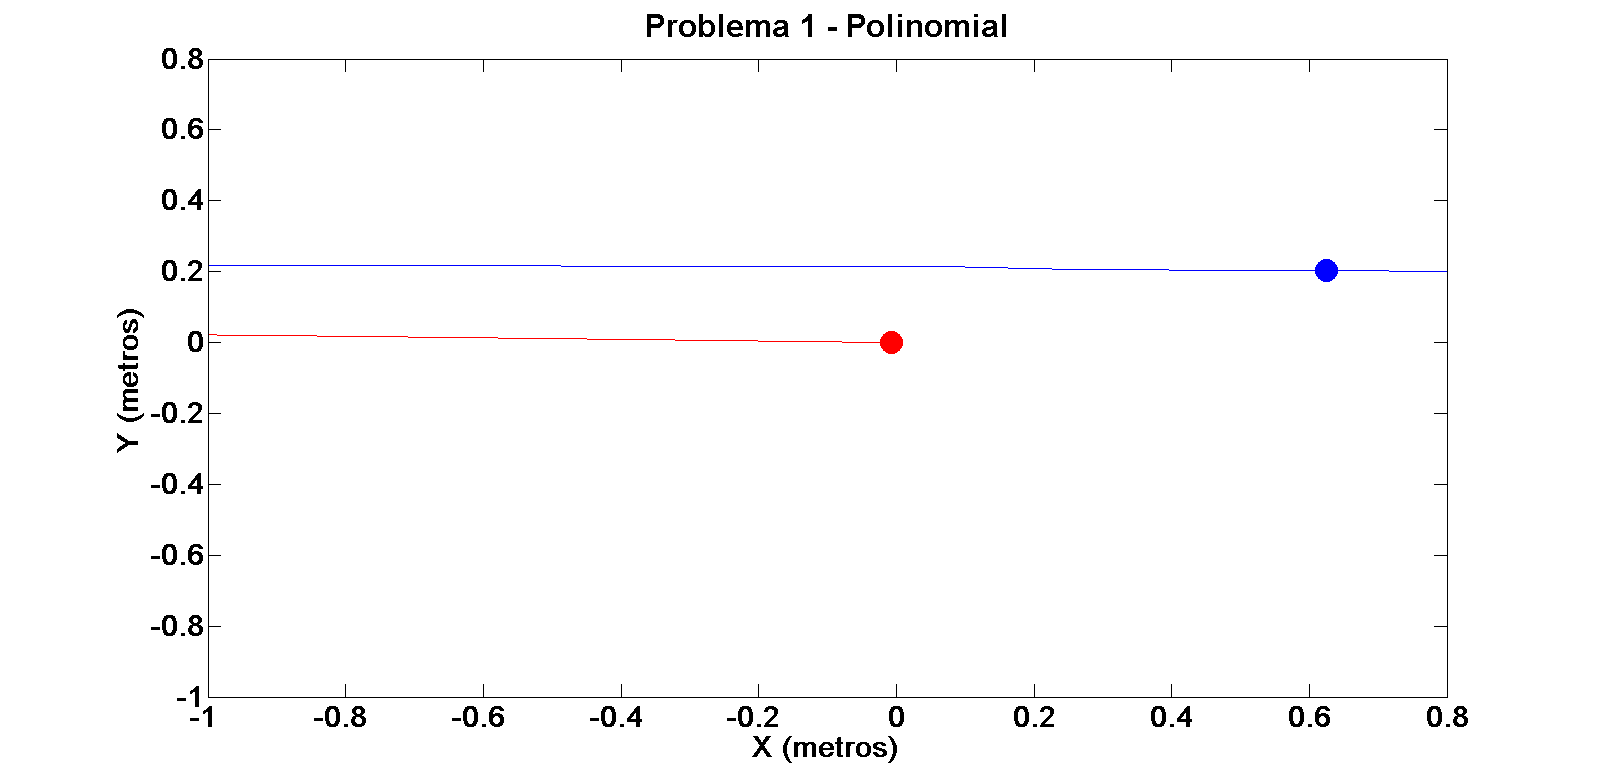
\includegraphics[width=.9\linewidth]{./Testes/Problema1/Polinomial/P1Antes}
		\caption{Sistema com Dois Robôs - Antes do alinhamento dos robôs}
		\label{fig:P12Ini}
	\end{subfigure}
	\begin{subfigure}{1.0\textwidth}
		\centering
		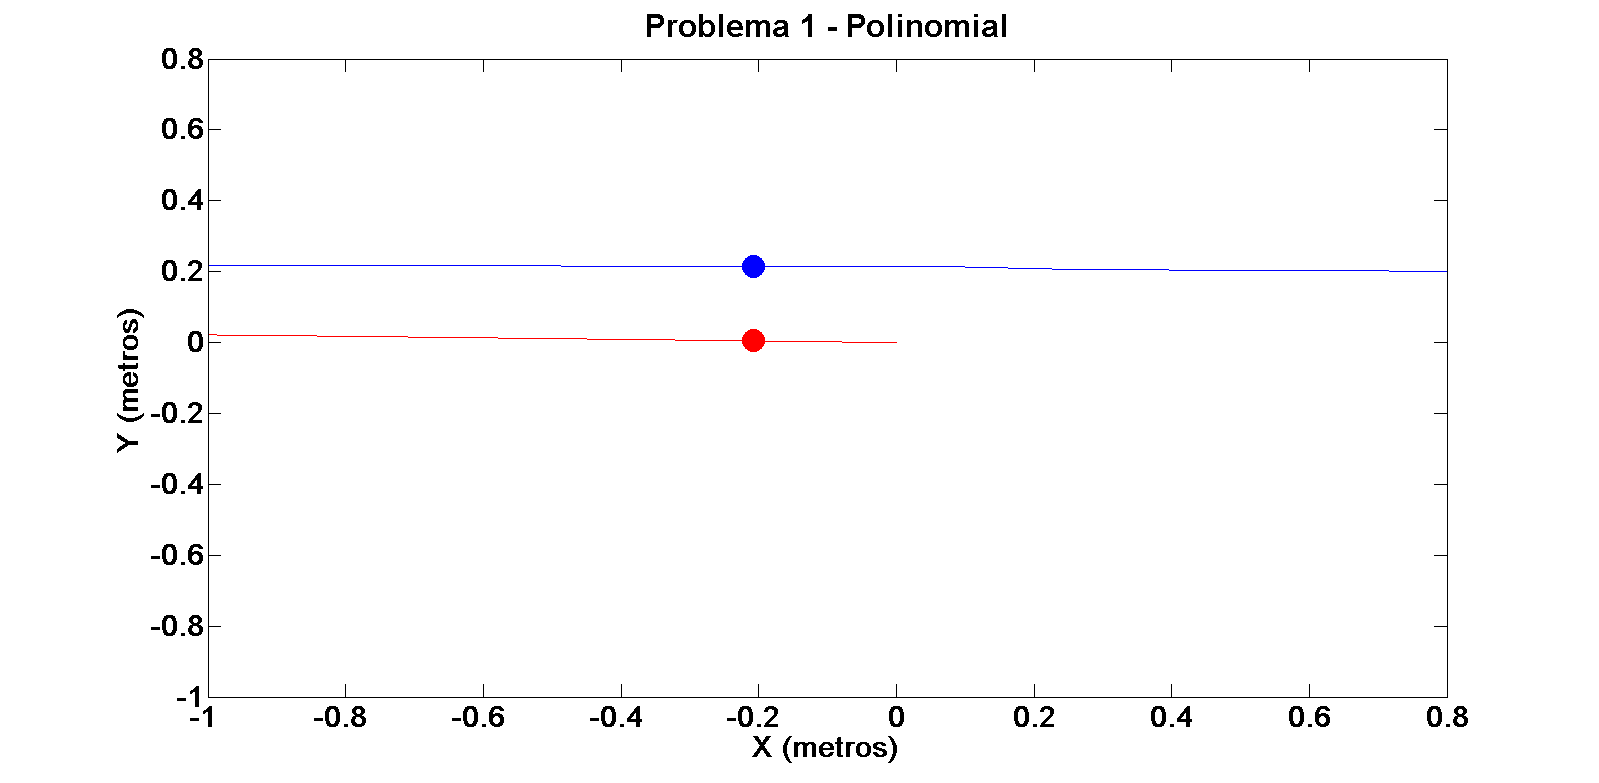
\includegraphics[width=.9\linewidth]{./Testes/Problema1/Polinomial/P1Depois}
		\caption{Sistema com Dois Robôs - Depois do alinhamento dos robôs}
		\label{fig:P12Fim}
	\end{subfigure}
	\caption{Problema 1 com 2 Robôs}
	\label{fig:sP12}
\end{figure}

\begin{figure}[!htb]
	\centering
	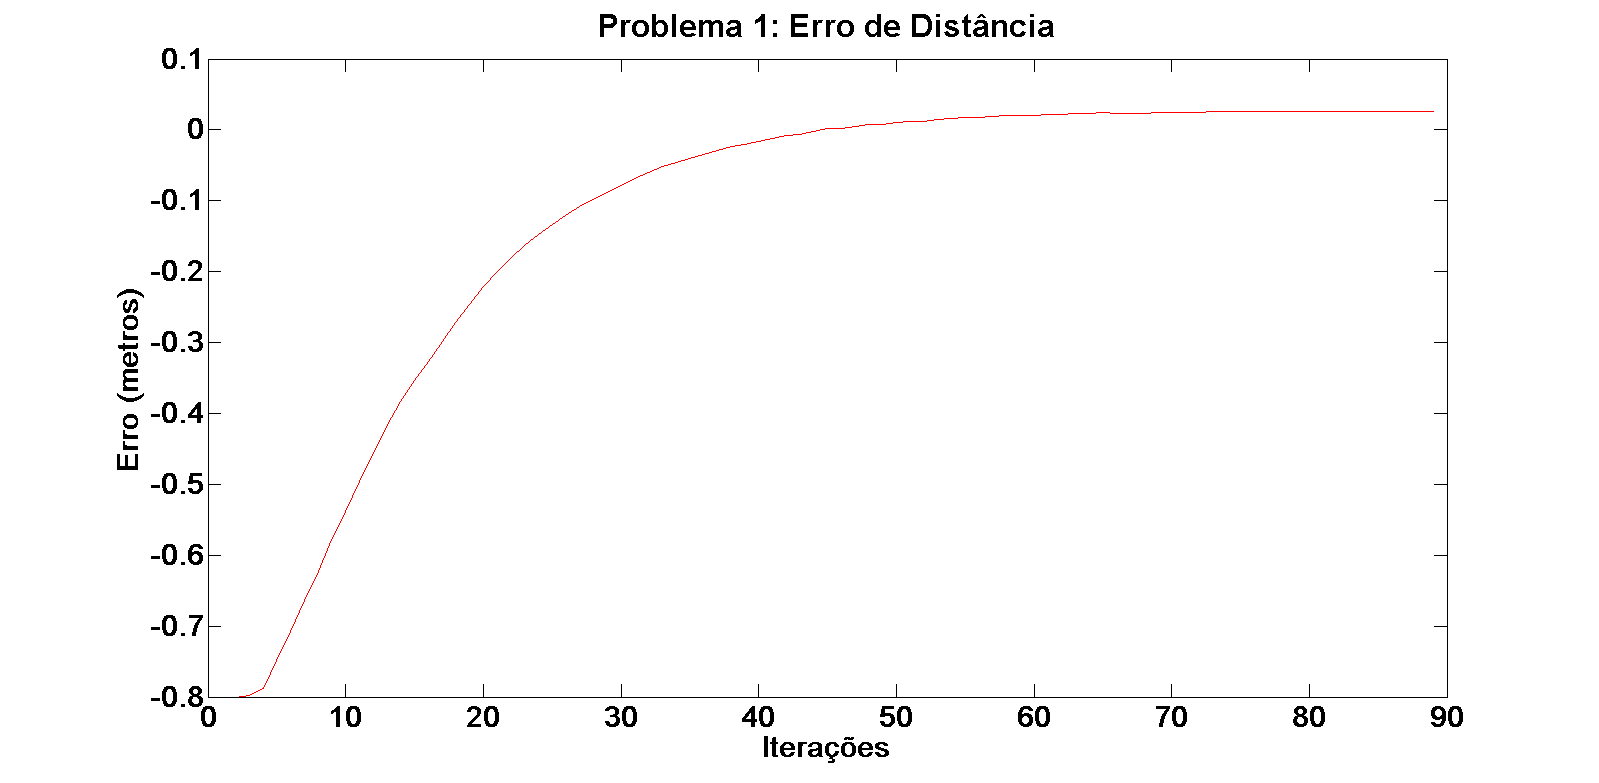
\includegraphics[width=.9\linewidth]{./Testes/Problema1/Incremental/ErroDistancia}
	\caption{Problema 1: Erro de Posição (x1 - x2)}
	\label{fig:P12Erro}
\end{figure}

\begin{figure}[!htb]
		\centering
		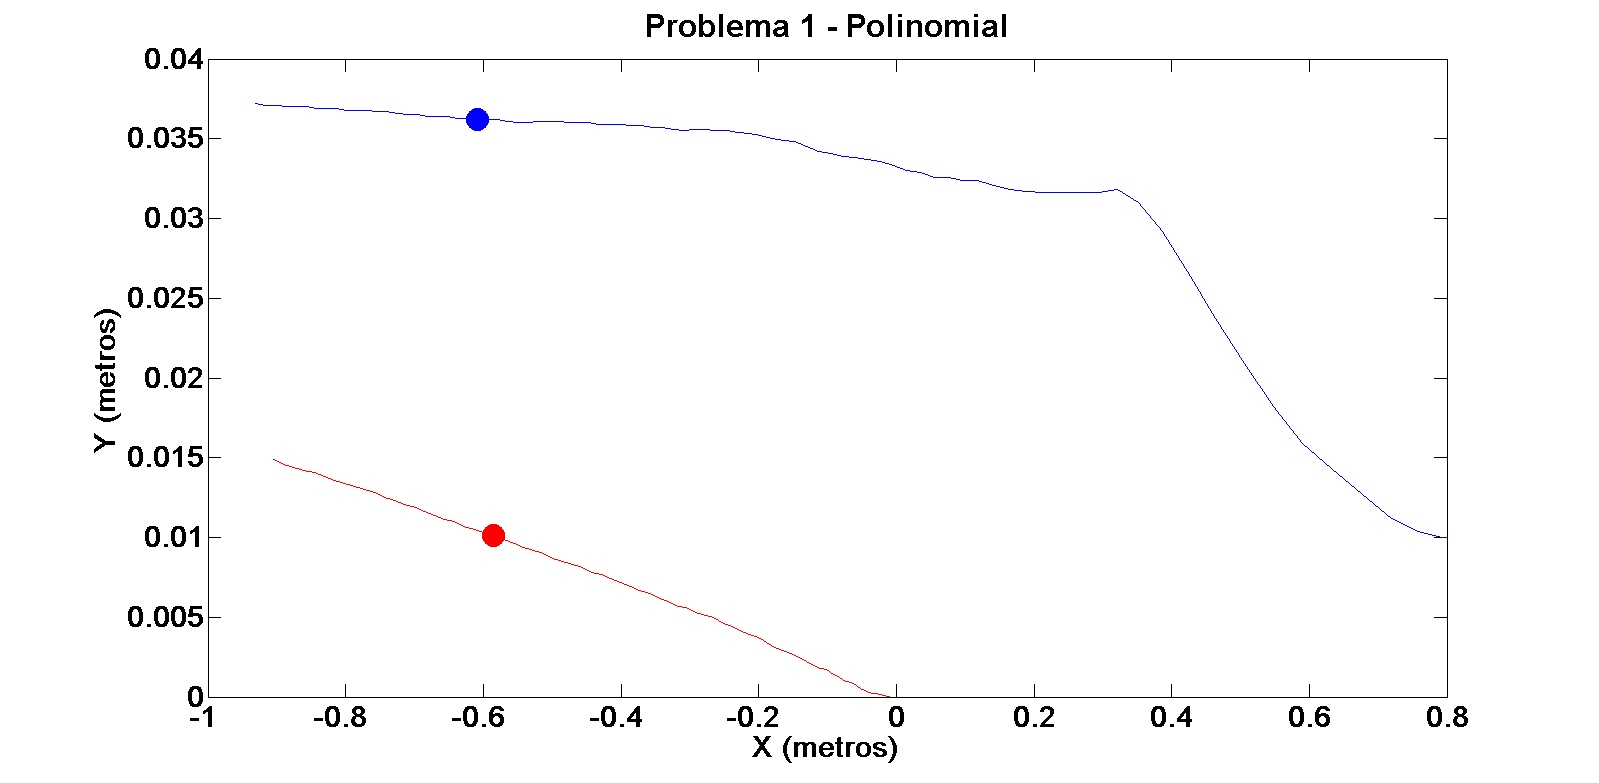
\includegraphics[width=.9\linewidth]{./Testes/Problema1/Incremental/P1Depois}
	\caption{Problema 1 com 2 Robôs: Deslocamento Lateral}
	\label{fig:sP13}
\end{figure}

O segundo problema consiste em fazer uma frota de \emph{N} robôs localizar e circundar um alvo a uma distância \emph{R} e em um determinado período \emph{T}, que deve variar de acordo com o tamanho da frota e os robôs devem ter a mesma distância entre eles. Após realizados todos os testes e simulações, aplicou-se a estratégia em uma frota de dois robôs, colocando-os a mesma distância do alvo e em sentidos opostos, de maneira que eles não se colidissem quando o sistema ainda não estivesse estável. 

Como pode ser visto na \autoref{eq:posDesejada_p2}, o cálculo da posição desejada para o segundo problema depende do tempo, devido a falta de sincronismo entre os relógios dos robôs, a posição desejada calculada pelos robôs pode apresentar erros na distribuição circular balanceada. Para contornar este problema, a solução encontrada foi passar para o outro robô o tempo do mestre. Desta forma, elimina-se o problema da falta de sincronismo entre os relógios. 

Como pode ser visto na \autoref{fig:P2}, a estratégia se mostrou plausível, visto que ambos os robôs convergiram para o alvo, contornando-o a uma distância de aproximadamente 30 centímetros, se mantiveram equidistantes e após a retirada de um dos robôs, %o período \emph{T} foi reduzido pela metade, 
dobrou-se o $\omega$ do robô, cobrindo melhor a fronteira. Para a realização deste experimento foi utilizado o controlador da malha interna polinomial e o controlador proporcional da malha intermediária de ganho 2 que obteve um resultado melhor, como demonstrado no \autoref{chap:testesMalhas}.

   \begin{figure}[!htb]
   	\centering
   	\begin{subfigure}{1.0\textwidth}
   		\centering
   		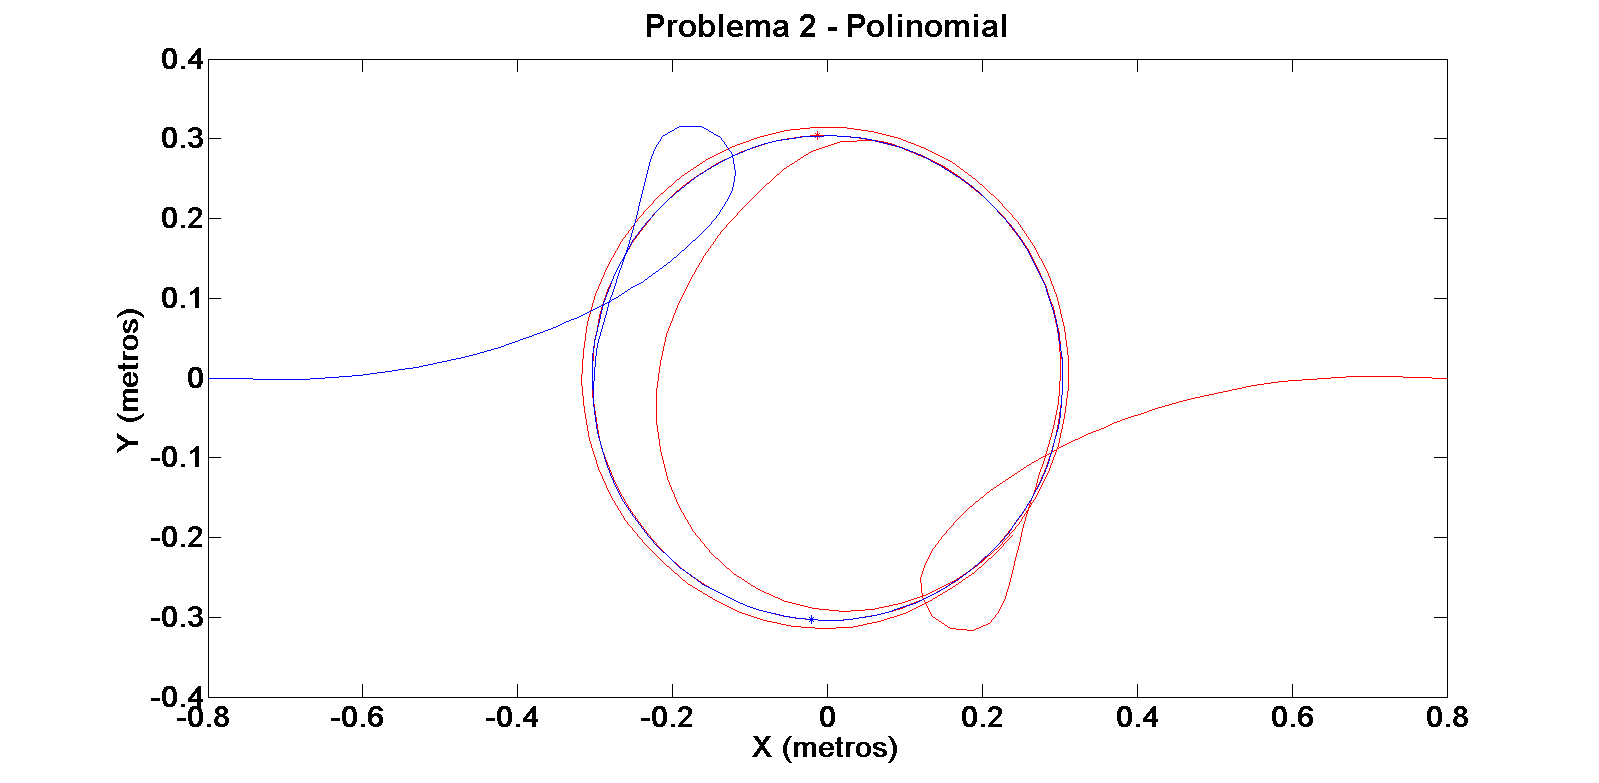
\includegraphics[width=.9\linewidth]{./Testes/Problema2/Incremental/2Rb}
   		\caption{Sistema com Dois Robôs}
   		\label{fig:P2Ini}
   	\end{subfigure}
   	\begin{subfigure}{1.0\textwidth}
   		\centering
   		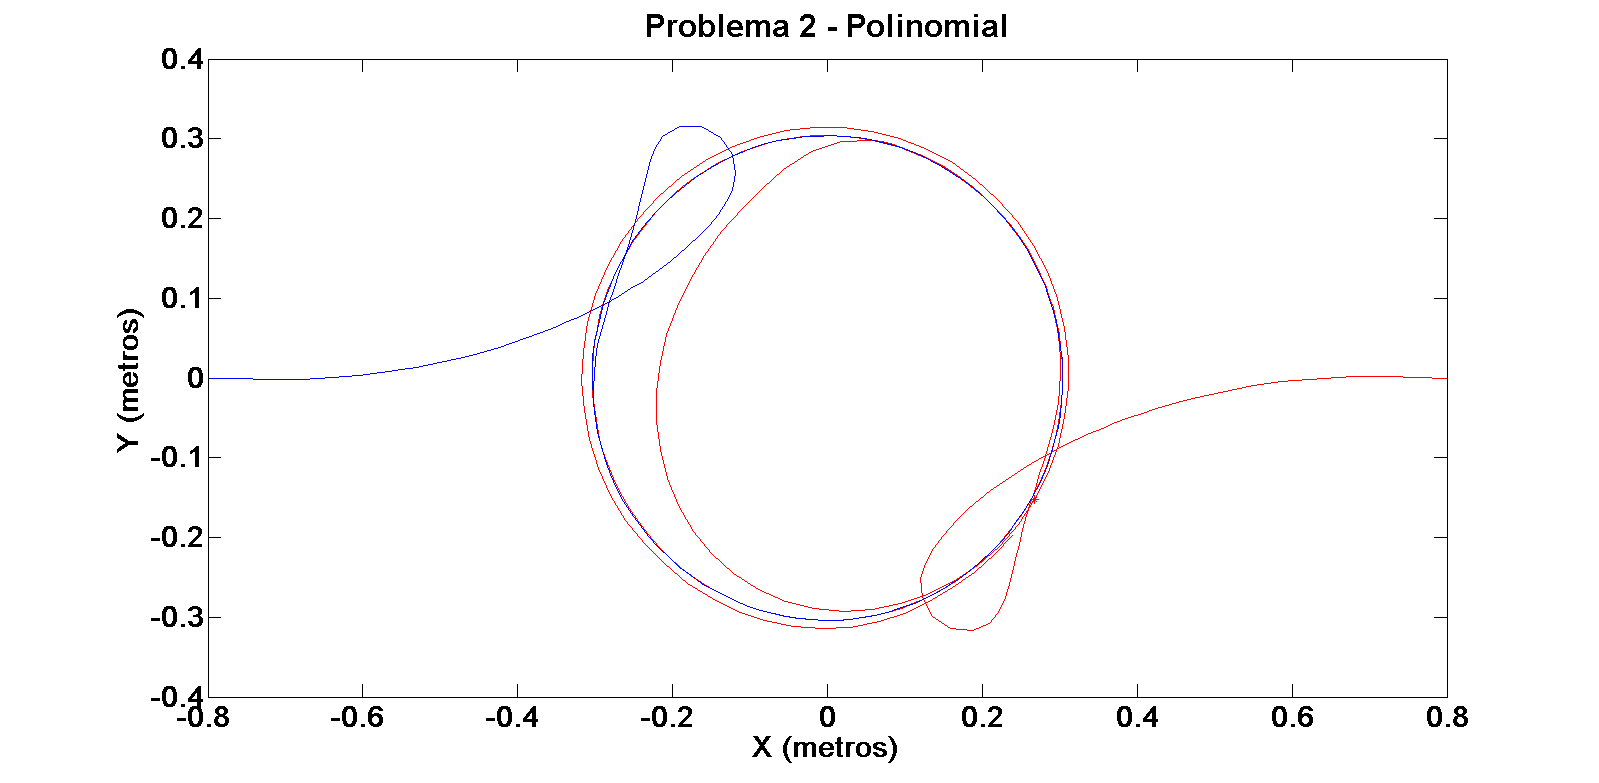
\includegraphics[width=.9\linewidth]{./Testes/Problema2/Incremental/1Rb}
   		\caption{Sistema com um Robô}
   		\label{fig:P2Fim}
   	\end{subfigure}
   	\begin{subfigure}{1.0\textwidth}
   	\centering
   	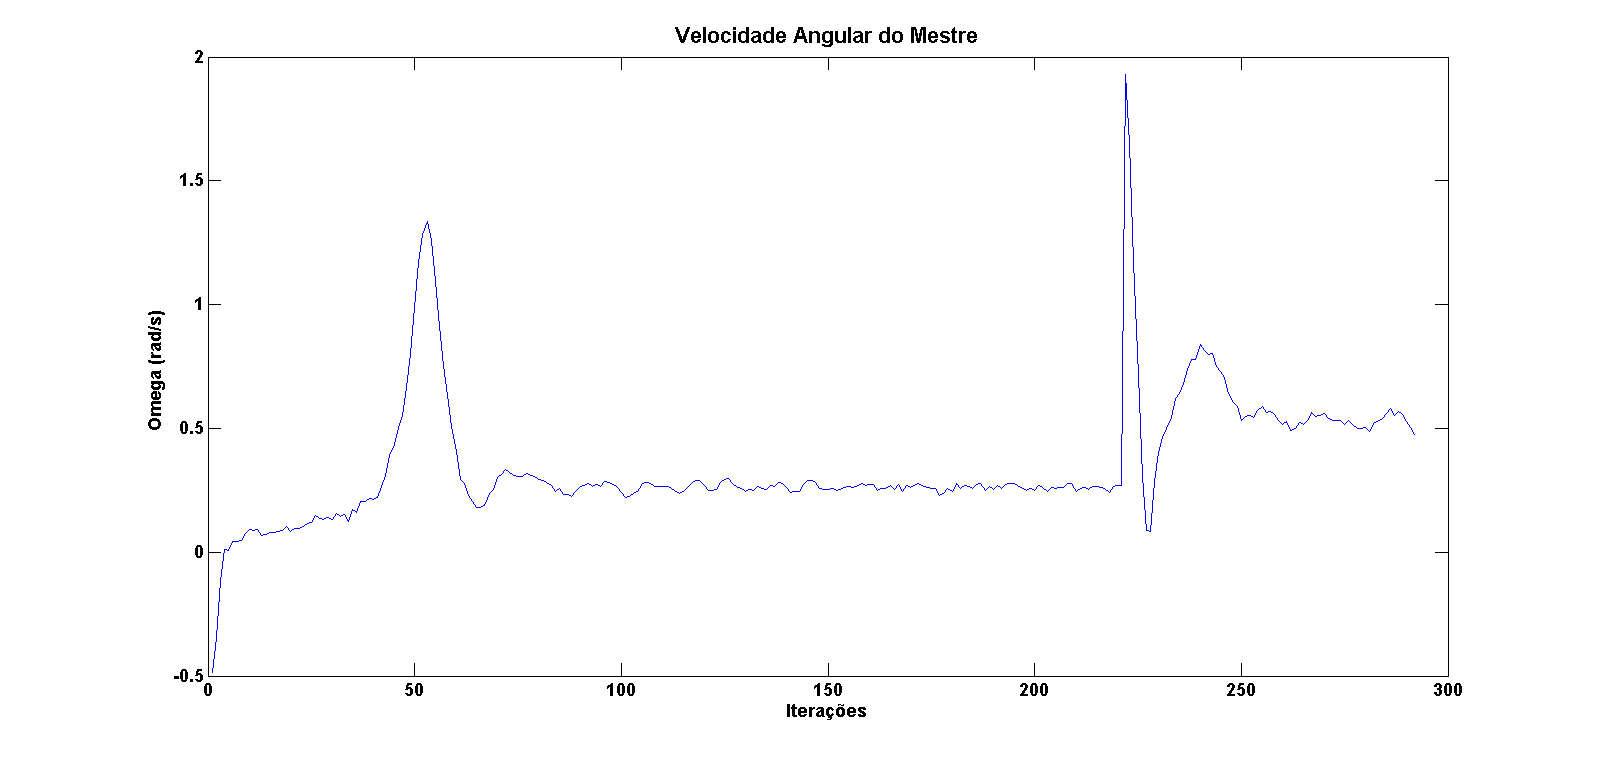
\includegraphics[width=.9\linewidth]{./Testes/Problema2/Incremental/velAng}
   	\caption{Velocidade Angular do Mestre}
   	\label{fig:P2velAng}
   \end{subfigure}
   	\caption{Segundo Problema com Falha de um dos Robôs}
   	\label{fig:P2}
   \end{figure}
   